\chapter{Introduction}
\label{ch:introduction}

This is the introduction. Here is a section.

\section{Your first section}

And this is a subsection.

\subsection{Your first subsection}

And here are some citations. First this \cite{kalouli2022negation}. (This is a citation in parenthesis \citealt{kalouli2022negation}). This is with a page number \citep[p. 5]{kalouli2022negation}. \citet{kalouli2022negation} says very smart things. Here are multiple citations from the same author in the same year: \citet{zymla2024ambiguity,Zymla2024}

\section{Figure example}

Here is an example figure:

\begin{figure}
    \centering
    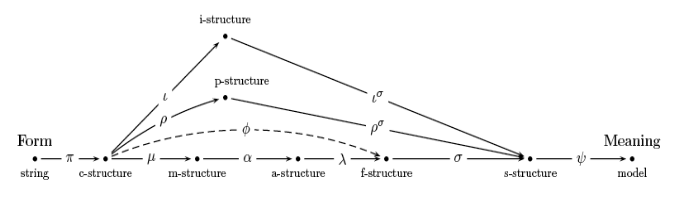
\includegraphics[scale=0.5]{./tex/figures/parallelprojection.png}
    \caption{This is the projection architecture}
    \label{fig-label1}
\end{figure}

Figure \ref{fig-label1} describes the projection architecture. 

\section{Linguistic exmaples}

You can refer to examples with \texttt{\\ref}. Like this \ref{ex:intro:ex1}.

\ex. \label{ex:intro:ex1} This is a simple linguistic example. 

\ex. Some text here 
\a. This is an example with subexamples
    \b. Second example


Here is an example with glossing.

\exg. The first line \\
    det first line \\
    \trans \textit{`The translation'}

\exg. The first line \\
    det {second first} line \\
    \trans \textit{`The translation'}

    This page explains linguistic examples: \url{https://ftp.tu-chemnitz.de/pub/tex/macros/latex/contrib/linguex/doc/linguex-doc.pdf}

    This sentence has a footnote.\footnote{This is a footnote.}

    \section{Tables}

    Go to \url{https://www.tablesgenerator.com/} to create tables:

    \begin{table}[]
    \centering
\begin{tabular}{l||ll}
a  & \multirow{3}{*}{b} & c  \\
1  &                    & 3  \\
ho &                    & ho
\end{tabular}
\caption{This is an example table}
\label{table:hohoho}
\end{table}

This is a reference to Table \ref{table:hohoho}

The tabular environment is sometimes useful if you require aligned elements.

\ex. \textbf{Basic template for gradable adjectives}
\a. \begin{tabular}{ll}
\textbf{modification:} & $\lambda P.\lambda Q.\lambda x.P(x) \land Q(x) : (e \to t) \to ((e \to t) \to e \to t)$ \\
\textbf{adjective:} & $\lambda \delta .\lambda x.degree(x,\delta) : d \to e \to t$\\
\textbf{pos:} & $\lambda P.\lambda \delta. \lambda x.P(\delta)(x) \land \theta_{adj} < \delta$ : $(d \to e \to t) \to d \to e \to t$ \\
\textbf{degree closure:} & $\lambda P_{dt}.\exists \delta [P(\delta)] : (d \to t) \to t$
\end{tabular}

\section{Switching between languages}

%requires babel/font encoding for cyrillic 
\selectlanguage{russian}

\ex. Это предложение на русском языке.

\selectlanguage{english}

\ex. Back to English.

\section{Special symbols}

Use \url{https://detexify.kirelabs.org/classify.html} to find special symbols

\section{Math mode}

Mathematical expressions are written in mathmode. Certain special symbols only work in math mode. Math mode is delimited by \$. Use \texttt{\\text/} to mix math symbols and text (e.g., for semantic expressions). Certain letters and symbols, e.g., $f$ and $-$ have a special type-setting in math mode.

\ex. \a. $\lambda x. \lambda y.\text{visit}(y,x): g \multimap (h \multimap f)$
\b. $afb-cde$
\c. $\text{afb-cde}$

\section{Minipages}

Minipages are one way to put things side by side.

\ex. \begin{minipage}[t]{.5\textwidth}
  This is column 1  
\end{minipage}%
\begin{minipage}[t]{.5\textwidth}
    This is column 2
\end{minipage}

Optionally you can use fbox to adjust the layout 

\ex. \fbox{\begin{minipage}[t]{.5\textwidth}
  This is column 1  
\end{minipage}}%
\fbox{
\begin{minipage}[t]{.5\textwidth}
    This is column 2
\end{minipage}
}

\newpage

\section{Code blocks}

\begin{figure}[h!]
\begin{center}
\begin{minipage}{.72\textwidth}
\begin{lstlisting}
{
    {
        {
        high : (g_d -o (g_e -o g_t))
        pos : ((g_d -o (g_e -o g_t)) -o (g_d -o (g_e -o g_t))) 
        }
    mod : ((g_e -o g_t) -o ((g_e -o g_t) -o (g_e -o g_t))) || noscope
    elephant : (g_e -o g_t)
    }
d-closure : ((g_d -o f_t) -o f_t)
some : ((g_e -o g_t) -o ((g_e -o f_t) -o f_t))
appear : (g_e -o f_t)
}


10: d-closure([/y1_d.some([/z1_e.mod([/z_e.pos([/x_d.[/y_e.high(x)(y)]])(y1)(z)])([/x1_e.elephant(x1)])(z1)])([/x2_e.appear(x2)])])
\end{lstlisting}
\end{minipage}
\end{center}
\vspace{-5mm}
\caption{Constraining ambiguities via bracketed proofs}
\label{fig:adj-comp-constrained}
\end{figure}

\section{AI support}

Ask ChatGPT for help: \url{https://chat-ai.academiccloud.de/}